\section{Introduction}

This chapter presents Stochastic Bi-Objective Beam Search (SBBS), a new decoding strategy inspired by \citet{holtzman2018learning}, to generate musical pieces conveying a target emotion. SBBS works by steering at generation time the probability distribution of a LM with the probabilities given by a music emotion classifier. Unlike the method presented in the previous chapter, SBBS does not update the weights of the LM to control it towards a target emotion. SBBS is proposed as part of a system called \textit{Bardo Composer}, or \textit{Composer} for short, to generate background piano music for tabletop role-playing games (TRPG). Composer is applied to score sessions of Dungeons and Dragons (D\&D), a TRPG in which the players interpret characters,
known as player characters (PCs), in a story told by the dungeon master (DM), a special player who also interprets all nonplayer characters (NPCs) in the story. Composers' goal is to augment the players' experience with soundtracks that match the story being told in the game. For example, if the players are fighting a dragon, Composer should generate a piece matching such a tense moment of the story. TRPG players often manually choose songs to play as background music to enhance their experience \cite{bergstrom2014case}. Therefore, the system should allow players to concentrate on the role-playing part of the game and not on the disruptive task of selecting the next music piece to be played.

Bardo Composer builds upon a previous system called \textit{Bardo} \cite{padovani2017}, which selects pre-authored background music for TRPGs. Bardo uses a \textit{naive bayes} approach to classify captions (sentences) produced by a speech recognition system into one of the four emotions: happy, calm, agitated, and suspenseful. Bardo then selects a music piece from a library corresponding to the classified emotion. The selected piece is then played as background music whenever the naive bayes classifier detects an emotion transition in the story.
As shown in Figure \ref{fig:bardo}, Composer has a similar structure as the previous system, with the major difference that Composer generates completely new pieces as opposed to select pre-authored ones. Composer also uses a speech recognition system to translate players' speeches into captions. However, unlike the previous system, Composer classifies the captions with a transformer according to a discrete circumplex model of emotion. A second transformer is trained to classify the emotion of symbolic piano pieces according to the same discrete circumplex model. Composer then uses SBBS to control a LM with the music emotion classifier to generate music pieces conveying the target emotion given by the story emotion classifier.

\begin{figure}[h]
\centering
 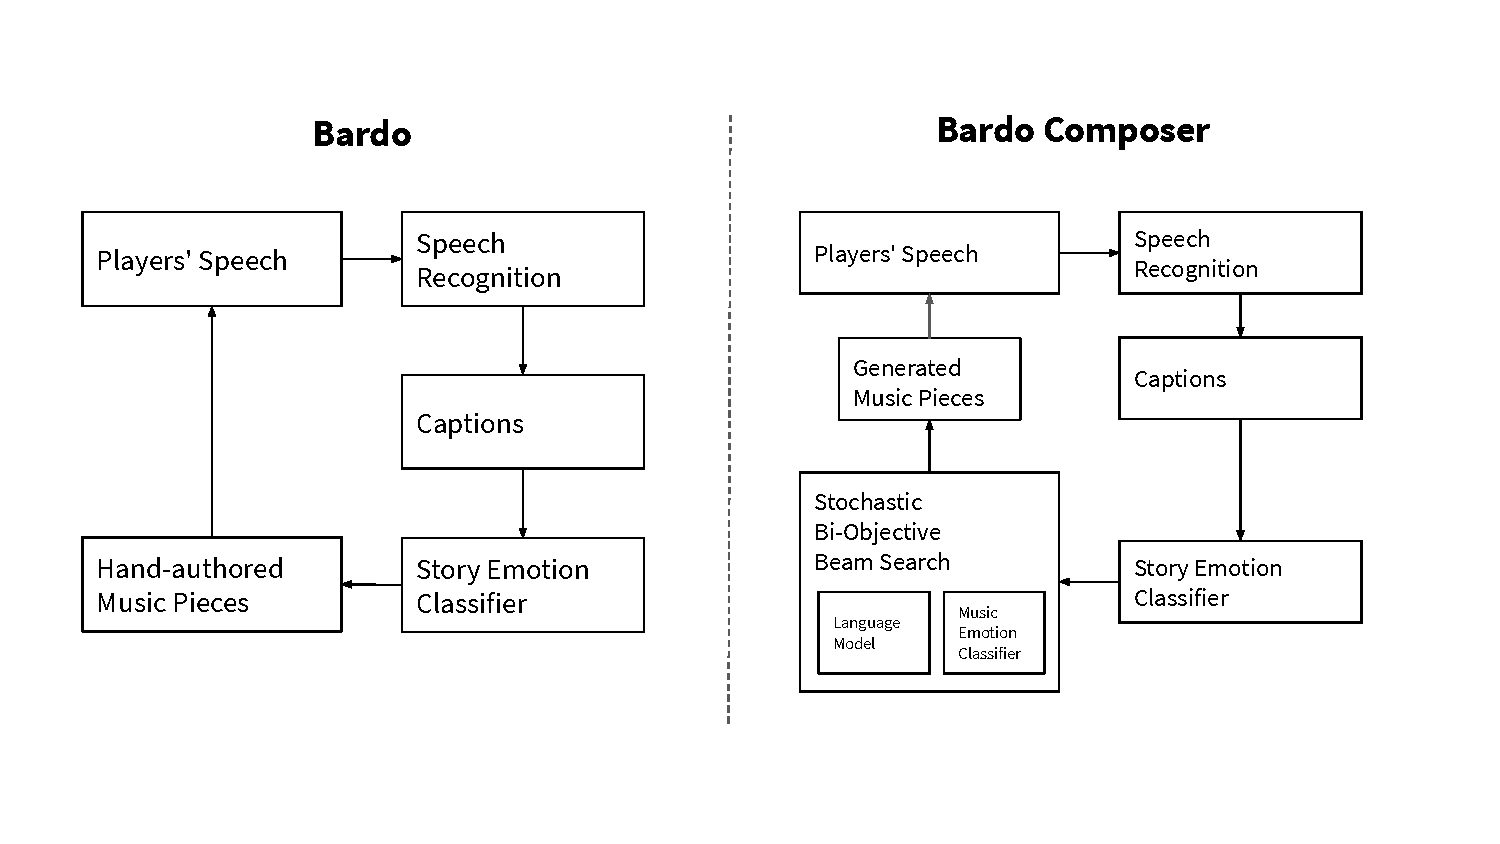
\includegraphics[width=\columnwidth]{imgs/aiide20/composer.pdf}
 \caption{Diagrams with the architecture of Bardo (left) and Composer (right). }
 \label{fig:bardo}
\end{figure}

Two new datasets have been created to support both Bardo and Composer \cite{padovani2017, ferreira2020computer}: \textit{Call of the Wild} (CotW) and \textit{ADL Piano Midi}. CotW is a dataset of transcribed captions from YouTube videos of a D\&D campaign. ADL Piano Midi is a large and diverse MIDI dataset with piano pieces extracted from the Lakh MIDI dataset \cite{raffel2016learning}. Moreover, in this work, the VGMIDI dataset has been extended from 95 to 200 labeled pieces using the same annotation method as the original dataset (see Chapter \ref{ch:ismir19}). All the 200 pieces are piano arrangements of video game soundtracks labeled according to the circumplex model of emotion. The discrete circumplex model of emotion used by Composer is defined to integrate emotions of the CotW stories with the VGMIDI pieces.

A listening test with 116 participants was performed to evaluate whether human subjects are able to correctly identify the emotion conveyed in pieces generated by Composer. Results showed that human subjects could correctly identify the emotion of the generated pieces as accurately as they were able to identify the emotion of pieces written by humans. The original Bardo was published in the Proceedings of the 13th AAAI Conference on Artificial Intelligence and Interactive Digital Entertainment (AIIDE17) \cite{padovani2017} and Bardo Composer in the Proceedings of AIIDE20 \cite{ferreira2020computer}.

\section{Datasets}

\subsection{Call of the Wild}

A new dataset called \textit{Call of the Wild} (CotW) was created to train the story emotion classifier of the original Bardo. This dataset includes 9 episodes of the CotW D\&D campaign available on YouTube, which sum a total of 4 hours, 39 minutes, and 24 seconds of gameplay. Each episode is an independent YouTube video with approximately 30 minutes played by the same 4 players (1 DM and 3 PCs). All videos were processed by the YouTube speech recognition system that generated the English captions from the speeches of the 4 players. This process yielded 5,892 sentences (45,247 words), which 3 different annotators labeled according to a categorical model with four emotions: happy, calm, agitated, and suspenseful. The annotation process assumed the PCs perspective in the story, as there could be moments that PCs and NPCs could experience different emotions. Should two annotators agree on the label of a sentence $s$, then $s$ is labeled according to the two annotators. One of the annotators watched the videos again to break the ties (sentences that each annotator attributed a distinct label for).

% Composer uses the labeled pieces of the VGMIDI dataset to train the music emotion classifier. In this work, the VGMIDI dataset was extended from 95 to 200 labeled pieces using the same annotation method of the original dataset (see Chapter \ref{ch:ismir19}). All the 200 pieces are piano arrangements of video game soundtracks labeled according to the circumplex model of emotion.
Composer's story emotion classifier is also trained with the CotW dataset. However, in order to have an integrated model of emotion between the CotW stories and the VGMIDI music pieces, Composer uses a discretized circumplex model of emotion \cite{russell1980circumplex} that generalizes the four emotion model used in Bardo \cite{padovani2017}. In Composer's emotion model, the dimensions of valence and arousal assume binary values $v \in [0, 1]$ and $a \in [0, 1]$, respectively. Valence measures sentiment and thus $v = 0$ means a negative emotion and $v = 1$ means a positive emotion. Arousal measures the energy of the emotion, and thus $a = 0$ means that the emotion has low energy, whereas $a = 1$ means that the emotion has high energy. With this discretized circumplex model, Bardo's four emotion model is mapped to the following emotions:

\begin{enumerate}
    \item Suspenseful is mapped to low valence and arousal ($v = 0, a = 0$).
    \item Agitated is mapped to low valence and high arousal ($v = 0, a = 1$).
    \item Calm is mapped to high valence and low arousal ($v = 1, a = 0$).
    \item Happy is mapped to high valence and arousal ($v = 1, a = 1$).
\end{enumerate}

This mapping is based on the circumplex model used to annotate the VGMIDI dataset. When human subjects annotated that dataset, they used a continuous circumplex model with labels defining a fixed set of discrete basic emotions (see Figure \ref{fig:annotation_main}). This mapping allows one to use the circumplex model with the labeled CotW dataset. For example, in the context of D\&D, the sentence ``Roll initiative'' is normally said at the beginning of battles and it can be considered $(v = 0, a = 1)$, once a battle is a negative (dangerous) moment with high energy. ``Roll initiative'' is normally classified as agitated in the CotW dataset \cite{padovani2017}.

\subsection{ADL Piano MIDI}

Composer trains its LM with a new dataset called ADL (Augmented Design Lab) Piano MIDI. This new dataset is based on the Lakh MIDI dataset \cite{raffel2016learning}, which is one of the largest MIDI collections publicly available. The Lakh MIDI dataset contains 45,129 unique MIDI files in which different versions of the same piece may occur. Only one version of each piece was kept. Given that Composer focuses on piano pieces, only the tracks with instruments from the piano family (MIDI program numbers 1-8 in the dataset) were considered from the Lakh MIDI dataset. This process yielded a total of 9,021 unique piano MIDI files. These files are mainly Rock and Classical pieces, so to increase genre diversity in the dataset (e.g., Jazz, Blues, and Latin), an additional 2,065 files were included from public sources on the Internet\footnote{\url{https://bushgrafts.com/midi/} and \url{http://midkar.com/jazz/}}. All files in the final collection were de-duped according to their MD5 checksum. The final dataset has 11,086 unlabeled MIDI piano pieces. The motivation to create this new dataset instead of using the unlabelled VGMIDI pieces is to have a considerably larger and varied symbolic music dataset to support better pre-trained LMs.

\section{Bardo Composer}

The general structure of Composer is formalized in Algorithm \ref{alg:bardo}. It receives as input a speech recognition system $S$, a story emotion classifier $E_s$, a music emotion classifier $E_m$, a LM for symbolic music generation $L$, a speech signal $p$ with the last sentences spoken by the players, and a sequence $x$ of musical symbols composed in previous calls to Composer. The algorithm also receives parameters $b$ and $k$, which are used in \texttt{SBBS} described in Algorithm \ref{alg:sbs}. Composer returns a symbolic piece that tries to match the emotion in the players' speeches. Composer starts by transcribing the speech signal $p$ into a caption $s$ with $S$ (line \ref{line:voice2text}). In addition to a caption, $S$ returns the duration $l$ of the signal $p$ in seconds. Then, Composer classifies the emotion of $s$ in terms of valence $v$ and arousal $a$ and it invokes \texttt{SBBS} to generate a sequence of symbols $y$ that matches the desired length $l$ and emotion with arousal $a$ and valence $v$. \texttt{SBBS} receives as input the models $L$ and $E_m$, the current sequence $x$, the desired emotion values $v$ and $a$, \texttt{SBBS}'s parameter values $b$ and $k$, and the desired length $l$ of the piece to be generated. %\texttt{SBBS} is described below.

\begin{algorithm}[h]
\caption{Bardo Composer}
\label{alg:bardo}
\begin{algorithmic}[1]
\REQUIRE Speech recognition system $S$, Text emotion classifier $E_s$, Music emotion classifier $E_m$, LM $L$, speech signal $p$, previously composed symbols $x$, beam size $b$, number of symbols $k$
\ENSURE Music piece $x$
\STATE $s, l \gets S(p)$ \label{line:voice2text}
\STATE $v, a \gets E_s(s)$ \label{line:emotion_classification}
% \STATE $x \gets \{\}$ \label{line:init}
%\STATE $i \gets 0$
%\WHILE{time of play of $[x_{t}, \cdots, x_{t + i}]$ is lower than $k$} \label{line:generation1}
\STATE $y \gets$ \texttt{SBBS}$(L, E_m, x, v, a, b, k, l)$ \# \emph{see Algorithm~\ref{alg:sbs}} \label{line:sbs}
\RETURN $x \cup y$ \label{line:generation2}
%\STATE $i \gets i + 1$
%\ENDWHILE
%\RETURN $x$
\end{algorithmic}
\end{algorithm}

In the first call to Composer, the sequence $x$ is initialized with the symbols of the first 4 timesteps of a random human-composed piece with the emotion $v, a$, as returned by $E_s$. Every time there is a transition from one emotion to another, the sequence $x$ is reinitialized using the same process. This is used to bias the generative process and to emphasize emotion transitions. To be used in real-time, Composer is invoked with the most recently captured speech signal $p$ and returns a composed piece of music. While the most recent piece is being played at the game table, Composer receives another signal $p$ and composes the next excerpt. One also needs to define the length of the signal $p$. Similar to Bardo \cite{padovani2017}, Composer uses YouTube's subtitle system as the speech recognition system $S$. Therefore, signals $p$ are long enough to form a sentence in the form of a caption.

\subsection{Story Emotion Classifier}

Composer's story emotion classifier $E_s$ is trained with a transfer learning approach, in which a pre-trained BERT$_{BASE}$ LM \cite{devlin2018bert} is fine-tuned with the CotW dataset. This transfer learning approach is used because the pre-trained BERT$_{BASE}$ LM has been shown to boost models' performance on a wide range of NLP tasks \cite{devlin2018bert}. BERT$_{BASE}$ uses transformer encoder blocks with 12 layers, 768 units per layer, and 12 attention heads. It was pre-trained with both the BooksCorpus dataset (800M words) \cite{zhu2015aligning} and the English Wikipedia (2,500M words). Although in Algorithm \ref{alg:bardo} the story emotion classifier is depicted as a single model $E_s$, in practice, Composer treats valence and arousal independently. Thus, BERT$_{BASE}$ is independently fine-tuned on the CotW dataset \cite{padovani2017} for each dimension of the circumplex model. Fine-tuning consists of adding a linear classification head on top of the pre-trained BERT$_{BASE}$ and training all layers (including the pre-trained ones) of the resulting model end-to-end.

\subsection{Language Model}

At the time Composer was proposed, there was no publicly available high-capacity LM pre-trained with large MIDI datasets for symbolic music modeling. Therefore, a high-capacity GPT-2 LM was pre-trained on the ADL Piano MIDI dataset. The GPT-2 LM has 4 layers (transformer blocks), a context size of 1024 tokens, 512 embedding units, 1024 hidden units, and 8 attention heads. Composer uses GPT-2 instead of BERT because GPT-2 is better suited for sequence generation than BERT.

To process MIDI files as sequences with the GPT-2 LM, Composer encodes a MIDI file by parsing all notes from the \texttt{NOTE\_ON} and \texttt{NOTE\_OFF} events in the MIDI. A note is defined as a set $z = (z_p, z_s, z_d, z_v)$, where $\{z_p \in \mathbb{Z} \vert 0 \leq z_p < 128 \}$ is the pitch number, $\{z_s \in \mathbb{Z} \vert z_s \geq 0 \}$ is the note starting time in timesteps,  $\{z_d \in \mathbb{Z} \vert 0 \leq z_d \leq 56\}$ is note duration in timesteps and $\{z_v \in \mathbb{Z} \vert 0 \leq z_v < 128 \}$ is the note velocity. Given a MIDI \texttt{NOTE\_ON} event, a note $z$ is parsed by retrieving the starting time $z_s$ (in seconds), the pitch number $z_p$ and the velocity $z_v$ from that event. To calculate the note duration $z_d$, the end time $z_e$ (in seconds) of the corresponding \texttt{NOTE\_OFF} event is retrieved. Thus, the note duration $z_d = \floor{t \cdot z_e} - \floor{t \cdot z_s}$ is computed from the  discretized durations $z_s$ and $z_e$, where $t$ is a parameter defining the sampling frequency of the timesteps. Composer derives a sequence $x = \{z_v^1, z_{d}^1, z_{p}^1, \cdots, z_v^n, z_{d}^n, z_p^n\}$ of tokens for a given MIDI file by (a) parsing all notes $z^i$ from the file, (b) sorting them by starting time $z_s^j$, and (c) concatenating their velocity $z_v^j$, duration $z_d^j$, and pitch $z_p^j$. Composer adds two special tokens \texttt{TS} and \texttt{END} in the sequence $x$, to mark the end of a timestep and the end of a piece, respectively.

This encoding yields a vocabulary $V$ of size $|V| = 314$, which is slightly greater than the size of the vocabulary used in Chapter \ref{ch:ismir19} (225 tokens). This increase comes from the extra number of note durations that can be represented in this new scheme. The main difference between these two schemes is that the new one does not encode tempo directly. The tempo of the pieces is implicitly encoded in the duration of the notes. Faster pieces have shorter notes, whereas slower pieces have longer notes. Moreover, the duration of the notes is not encoded as a duration type, as in Chapter \ref{ch:ismir19}. In this new scheme, the duration is represented as the number of time steps that note lasts. The main motivation for this new scheme is to provide a more accurate representation of note durations without considerably increasing the size of the vocabulary.

\subsection{Music Emotion Classifier}

As was the case with $E_s$, the emotion music classifier $E_m$ is also trained with a transfer learning approach. $E_m$ fine-tunes the GPT-2 LM pre-trained on the ADL Piano MIDI dataset. Similar to $E_s$, $E_m$ also treats valence and arousal independently. Thus, the pre-trained GPT-2 is fine-tuned on the extended VGMIDI dataset for each dimension of the circumplex model. Following the approach of \citet{Radford2018}, these models were fine-tuned by adding and extra layer to the pre-trained LM and training the entire model (including the pre-trained layers) with the VGMIDI dataset \cite{ferreira_2019}.

\subsection{Stochastic Bi-Objective Beam Search}

Composer uses a new search-based decoding algorithm called \textit{Stochastic Bi-Objective Beam Search} (\texttt{SBBS}), which combines a LM and a music emotion classifier to bias the process of music generation to match a target emotion (line \ref{line:sbs} of Algorithm \ref{alg:bardo}). Given a LM $L$ and the music emotion classifiers $E_{m, v}$ and $E_{m, a}$, for valence and arousal, respectively, the goal of \texttt{SBBS} is to allow for the generation of pieces that sound ``good'' (i.e., have high probability value according to the trained LM), but that also match the current emotion of the story being told by the players. \texttt{SBBS} is stochastic because it samples from a distribution instead of greedily selecting the best sequences of symbols, as a regular beam search does. The regular beam search is deterministic and so it always generate the same piece for a given input sequence $x$ and emotion ($v,a$). The stochasticity of \texttt{SBBS} allows it to generate different music pieces given the same input parameters $x$ and ($v, a$). \texttt{SBBS} is ``bi-objective'' because it optimizes for realism and emotion. Algorithm \ref{alg:sbs} shows \texttt{SBBS}'s pseudocode. The letters $x, y$, and $m$ denote sequences of musical symbols. Function $p_L(y) = \prod_{y_t \in y} P(y_t|y_1, \cdots, y_{t-1})$ is the probability of sequence $y$ according to the LM $L$; a high value of $p_L(y)$ means that $y$ is recognized as a piece of ``good quality'' by $L$. Function $l(y)$ denotes the duration in seconds of piece $y$. Finally, $x[i:j]$ denotes the subsequence of $x$ starting at index $i$ and finishing at index $j$.

\begin{algorithm}[!h]
\caption{Stochastic Bi-Objective Beam Search}
\label{alg:sbs}
\begin{algorithmic}[1]
\REQUIRE Music emotion classifier $E_m$, LM $L$, previously composed symbols $x$, valence and arousal values $v$ and $a$, number $k$ of symbols to consider, beam size $b$, length $l$ in seconds of the generated piece.
\ENSURE Sequence of symbols of $l$ seconds.
\STATE $B \gets [x]$, $j \gets 0$ \label{line:sbs:init}
\WHILE{$l(y[t:t+j]) < l$, $\forall y \in B$} \label{line:sbs:stopping_condition}
    \STATE $C \gets \{\}$ \label{line:sbs:init_while}
    \FORALL{$m \in B$}
        \STATE $C_m \gets \{m \cup s \vert s \in V\}$ \label{line:sbs:children}
        \STATE $C_k \gets k$ elements $y$ from $C_m$ with largest $p_L(y)$ \label{line:sbs:pruning_model}
        \STATE $C \gets C \cup C_k$ \label{line:sbs:total_children}
    \ENDFOR
    \STATE $B \gets b$ sequences $y$ sampled from $C$ proportionally to $p_L(y) (1 - |v - E_{m,v}(y)|) (1 - |a - E_{m,a}(y)|)$ \label{line:sbs:sample_next_beam}
    \STATE $j \gets j + 1$ \label{line:sbs:end_while}
\ENDWHILE
\RETURN $m \in B$ such that $p_L(m) = \max_{y \in B}p_L(y)$ and $l(y[t: t+j]) \geq l$ \label{line:sbs:return}
\end{algorithmic}
\end{algorithm}

\texttt{SBBS} initializes the beam structure $B$ with the sequence $x$ passed as input (line \ref{line:sbs:init}).
\texttt{SBBS} also initializes variable $j$ for counting the number of symbols added by the search. \texttt{SBBS} keeps in memory at most $b$ sequences and, while all sequences are shorter than the desired duration $l$ (line \ref{line:sbs:stopping_condition}), it adds a symbol to each sequence (lines \ref{line:sbs:init_while}--\ref{line:sbs:end_while}). In line \ref{line:sbs:init_while},
\texttt{SBBS} initializes a set $C$ to store the candidate solutions of the next beam structure $B$.
\texttt{SBBS} then generates all sequences by adding one symbol from vocabulary $V$ to each sequence $m$ from $B$ (line \ref{line:sbs:children}). These extended sequences, known as the children of $m$, are stored in $C_m$. The operations performed in lines \ref{line:sbs:pruning_model} and \ref{line:sbs:sample_next_beam} attempt to ensure the generation of good pieces that convey the desired emotion. In line \ref{line:sbs:pruning_model}, \texttt{SBBS} selects the $k$ sequences with the largest $p_L$-values among the children of $m$. This is because some of the children with low $p_L$-value could be attractive from the perspective of the desired emotion and, although the resulting piece could convey the desired emotion, the piece would be of low quality according to the LM. The best $k$ children of each sequence in the beam are added to set $C$ (line \ref{line:sbs:total_children}). Then, in line \ref{line:sbs:sample_next_beam}, \texttt{SBBS} samples the sequences that will form the beam of the next iteration. Sampling occurs proportionally to the values of $p_L(y) (1 - |v - E_{m,v}(y)|) (1 - |a - E_{m,a}(y)|)$, for sequences $y$ in $C$. A sequence $y$ has higher chance of being selected if $L$ attributes a high probability value to $y$ and if the music emotion model classifies the values of valence and arousal of $y$ to be similar to the desired emotion. When at least one of the sequences is longer than the desired duration of the piece, \texttt{SBBS} returns the sequence with largest $p_L$-value that satisfies the duration constraint (line~\ref{line:sbs:return}).

\section{Empirical Evaluation}

SBBS is empirically evaluated with two experiments. The first one evaluates the accuracy of the models for story and music emotion classification. The fine-tuned BERT$_{BASE}$ model for story emotion classification is compared against the simpler Na\"ive Bayes approach used in the original Bardo \cite{padovani2017}. The fine-tuned GPT-2 model for music emotion classification is compared against the simpler fine-tuned mLSTM presented in Chapter \ref{ch:ismir19}. The second experiment evaluates, with a listening test, whether human subjects can recognize different emotions in pieces generated by Composer for the CotW campaign.

\subsection{Emotion Classifiers}

\subsubsection{Story Emotion}

The story emotion classifier is a pair of BERT$_{BASE}$ models, one for valence and one for arousal.
Both these models were fine-tuned for 10 epochs with the Adam optimizer \cite{adam14}. Each training step was performed over a mini-batch of size 32. The learning rate was set to 3e-5 and the dropout rate to 0.5. The CotW dataset is divided into 9 episodes. Thus, the accuracy of each BERT$_{BASE}$ classifier is evaluated with a leave-one-out strategy. Given a set of episodes $E$, for each episode $e \in E$, the $E - e$ episodes are used for training, and the episode $e$ is used for testing. For example, when testing on episode 1, episodes 2-8 are used for training. Every sentence is encoded using a WordPiece embedding \cite{wu2016google} with a 30,000 token vocabulary.

The fine-tuned BERT$_{BASE}$ classifiers are compared with Bardo's Naive Bayes (NB) approach, which encodes sequences using bag-of-words with tf–idf. Table \ref{tab:valence} shows the accuracy of the valence classification of both these methods per episode. The BERT$_{BASE}$ classifier outperforms NB in all the episodes, having an average accuracy 7\% higher. For valence classification, the hardest episode for both the models is episode 7, where BERT$_{BASE}$ had the best performance improvement when compared to NB. Episode 7 is different from all other episodes. While the other episodes are full of battles and ability checks, episode 7 is mostly PCs talking with NPCs. Therefore, what is learned in the other episodes does not generalize well to episode 7. The improvement in accuracy of BERT$_{BASE}$ in that episode is likely due to the model's pre-training. Episodes 5 and 9 were equally easy for both methods because these episodes are similar to one another. What is learned in one of these episodes generalizes well to the other.

\begin{table}[!h]
\centering
%\tiny
%\small
\setlength{\tabcolsep}{4pt}
\begin{tabular}{crrrrrrrrrr}
%\cline{2-11}
\toprule
\multirow{2}{*}{\textbf{Alg.}} & \multicolumn{9}{c}{\textbf{Episodes}} & \multirow{2}{*}{\textbf{Avg.}} \\
\cmidrule{2-10}
& \multicolumn{1}{c}{\textbf{1}}   & \multicolumn{1}{c}{\textbf{2}}   & \multicolumn{1}{c}{\textbf{3}}  & \multicolumn{1}{c}{\textbf{4}} & \multicolumn{1}{c}{\textbf{5}}  & \multicolumn{1}{c}{\textbf{6}}  & \multicolumn{1}{c}{\textbf{7}} & \multicolumn{1}{c}{\textbf{8}}  & \multicolumn{1}{c}{\textbf{9}} &    \\
\midrule
\multicolumn{1}{l}{\textbf{NB}}   &   73 & 88  &  91 & 85   &  94 & 81  &  41 & 74   & 94    &   80 \\
\multicolumn{1}{l}{\textbf{BERT$_{BASE}$}}   &  \textbf{89}  & \textbf{92}  & \textbf{96}  &  \textbf{88} & \textbf{97}   & \textbf{81} & \textbf{66}   &  \textbf{83}   &  \textbf{96} &  \textbf{87}  \\
\bottomrule
\end{tabular}
\caption{Valence accuracy in percentage of Naive Bayes (NB) and BERT$_{BASE}$ for story emotion classification.}
\label{tab:valence}
\end{table}

Table \ref{tab:arousal} shows the accuracy of arousal classification of both NB and BERT$_{BASE}$. Again BERT$_{BASE}$ outperforms NB in all the episodes, having an average accuracy 5\% higher. In contrast with the valence results, here there is no episode in which BERT$_{BASE}$ substantially outperforms NB.

\begin{table}[!h]
\centering
%\tiny
%\small
\setlength{\tabcolsep}{4pt}
\begin{tabular}{crrrrrrrrrr}
%\cline{2-11}
\toprule
\multirow{2}{*}{\textbf{Alg.}} & \multicolumn{9}{c}{\textbf{Episodes}} & \multirow{2}{*}{\textbf{Avg.}} \\
\cmidrule{2-10}
& \multicolumn{1}{c}{\textbf{1}}   & \multicolumn{1}{c}{\textbf{2}}   & \multicolumn{1}{c}{\textbf{3}}  & \multicolumn{1}{c}{\textbf{4}} & \multicolumn{1}{c}{\textbf{5}}  & \multicolumn{1}{c}{\textbf{6}}  & \multicolumn{1}{c}{\textbf{7}} & \multicolumn{1}{c}{\textbf{8}}  & \multicolumn{1}{c}{\textbf{9}} &    \\
\midrule
\multicolumn{1}{l}{\textbf{NB}}  & 82 & 88  &  75 & 79   &  82 & 76  &  98 & 86   & 84    &   83 \\
\multicolumn{1}{l}{\textbf{BERT}}   &  \textbf{86}  & \textbf{90}  & \textbf{77}  &  \textbf{86} & \textbf{89}   & \textbf{88} & \textbf{99}   &  \textbf{90}   &  \textbf{88} &  \textbf{88}  \\
\bottomrule
\end{tabular}
\caption{Arousal accuracy in percentage of Naive Bayes (NB) and BERT$_{BASE}$ for story emotion classification.}
\label{tab:arousal}
\end{table}

\subsubsection{Music Emotion}

The music emotion classifier is a pair of GPT-2 models, one for valence and one for arousal. First, a GPT-2 LM is pre-trained with the new ADL Piano MIDI dataset. Each piece $p$ of this dataset is augmented by (a) transposing $p$ to every key, (b) increasing and decreasing $p$'s tempo by 10\%, and (c) increasing and decreasing the velocity of all notes in $p$ by 10\% \cite{oore2017learning}. Thus, each piece generated $12 \cdot 3 \cdot 3 = 108$ different examples. The pre-trained GPT-2 LM is then fine-tuned twice on the VGMIDI dataset, once for valence and once for arousal. It is important to highlight that the pieces used to pre-train the LM can be safely augmented because they are unlabelled. The labeled pieces are not augmented because that could affect the valence or arousal of the pieces.

Similar to the story emotion classifiers, the GPT-2 classifiers are fine-tuned for 10 epochs using an Adam optimizer with a learning rate of 3e-5. Unlike the story emotion classifiers, each training step is performed over mini-batches of size 16 (due to GPU memory constraints) and dropout of 0.25. The VGMIDI dataset is defined with training and testing splits of 160 and 40 pieces, respectively. Each piece $p$ of this dataset was augmented by slicing $p$ into 2, 4, 8, and 16 parts of equal length and emotion. Thus, each part of each slicing generated one extra example. This augmentation is intended to help the classifiers generalize for pieces with different lengths.

The fine-tuned GPT-2 classifiers are compared with mLSTM models that are also pre-trained with the ADL Piano Midi dataset and fine-tuned with the VGMIDI dataset. These baselines were chosen because they are currently the state-of-the-art models in the VGMIDI dataset \cite{ferreira_2019}. The mLSTMs have the same size as the GPT-2 models (4 hidden layers, 512 embedding units, 1024 hidden units) and are pre-trained and fine-tuned with the same hyper-parameters. Table \ref{tab:sent_accuracy} shows the accuracy of both models for valence and arousal. The performance of these models without pre-training (i.e., trained only on the VGMIDI dataset) is also reported. These are the baseline versions of the models.

\begin{table}[h!]
    \centering
    % \setlength{\tabcolsep}{4pt}
    \begin{tabular}{ccc}
    \toprule
    \textbf{Algorithm} & \textbf{Valence} & \textbf{Arousal} \\
    \midrule
    Baseline mLSTM & 69 & 67 \\
    Fine-tuned mLSTM & 74 & 79 \\
    Baseline GPT-2 & 70 & 76 \\
    Fine-tuned GPT-2 & \textbf{80} & \textbf{82} \\
    \bottomrule
    \end{tabular}
    \caption{Accuracy in percentage of both the GPT-2 and mLSTM models for music emotion classification. }
    \label{tab:sent_accuracy}
\end{table}

Results show that using transfer learning can substantially boost the performance of both the GPT-2 and the mLSTM. The fine-tuned GPT-2 is 10\% more accurate than its respective baseline in terms of valence and 8\% in terms of arousal. The fine-tuned mLSTM is 5\% more accurate than its respective baseline in terms of valence and 12\% in terms of arousal. Finally, the fine-tuned GPT-2 outperformed the fine-tuned LSTM by 6\% and 3\% in terms of valence and arousal, respectively.

\subsection{Listening Test}

Composer's performance in generating music that matches the emotions of a story is assessed with a listening test. Composer is applied to generate a piece for a snippet composed of 8 contiguous sentences of each of the first 5 episodes of the CotW dataset. Each snippet has one emotion transition that happens in between sentences. The sentences are 5.18 seconds long on average. To test Composer's ability to generate music pieces with emotion changes, human subjects were asked to listen to the 5 generated pieces and evaluate the transitions of emotion in each generated piece. The listening test was performed via Amazon Mechanical Turk and had an expected completion time of approximately 10 minutes. A reward of USD \$1 was given to each participant who completed the study.

In the first section of the study, the participants were presented with an illustrated description of the circumplex model of emotion and listened to 4 examples of labeled pieces from the VGMIDI dataset. Each piece had a different emotion: low valence and arousal, low valence and high arousal, high valence and low arousal, high valence and arousal. In the second section of the study, participants were asked to listen to the 5 generated pieces (one per episode). After listening to each piece, participants had to answer 2 questions: (a) ``What emotion do you perceive in the 1st part of the piece?'' and (b) ``What emotion do you perceive in the 2nd part of the piece?'' To answer these two questions, participants selected one of the four emotions: low valence and arousal, low valence and high arousal, high valence and low arousal, high valence and arousal. Subjects were allowed to play the pieces as many times as they wanted before answering the questions.
The final section of the study was a demographics questionnaire including ethnicity, first language, age, gender, and experience as a musician. To answer the experience as a musician, the participants used a 5-point Likert scale where 1 means ``I've never studied music theory or practice'' and 5 means ``I have an undergraduate degree in music''.

Composer is compared with a baseline method that selects a random piece from the VGMIDI dataset whenever there is a transition of emotion. The selected piece has the same emotion of the sentence (as given by the story emotion classifier). A between-subject strategy was used to compare these two methods, where Group $A$ of 58 participants evaluated the 5 pieces generated by Composer and Group $B$ of 58 participants evaluated the 5 pieces from the baseline. This strategy was used to avoid possible learning effects where subjects could learn emotion transitions from one method and apply the same evaluation directly to the other method. The average age of groups $A$ and $B$ are 34.96 and 36.98 years, respectively. In Group $A$, 69.5\% of the participants are male and 30.5\% are female. In Group $B$, 67.2\% are male and 32.8\% are female. The average musicianship of the groups $A$ and $B$ are 2.77 and 2.46, respectively.

Table \ref{tab:user_study} shows the results of the listening test. The two parts (p1 and p2 in the table) of each episode are considered independent pieces. The table presents the percentage of participants that correctly identified the pieces' valence and arousal (\textit{v} and \textit{a} in the table, respectively), as intended by the methods. This percentage is refeered to as the approach's accuracy. For example, 87\% of the participants correctly identified the arousal value that Composer intended the generated piece for part p1 of episode 4 (e4-p1) to have. The approaches' average accuracy is also presented across all pieces (\textit{Average} in the table) in terms of valence, arousal, and jointly for valence and arousal (\textit{va} in the table). The \textit{va}-value of 34 for Composer means that 34\% of the participants correctly identified the system's intended values for valence and arousal across all pieces generated.

\begin{table}[!h]
\centering

%\small
\resizebox{\columnwidth}{!}{
\setlength{\tabcolsep}{3pt}
\begin{tabular}{crrrrrrrrrrrrrrrrrrrrrrr}
%\cline{2-11}
\toprule
\multirow{3}{*}{\textbf{Method}} & \multicolumn{20}{c}{\textbf{Episodes}} & \multicolumn{3}{c}{\multirow{3}{*}{\textbf{Average}}} \\
\cmidrule{2-21}
% & \multicolumn{4}{c}{\textbf{1}} & \multicolumn{4}{c}{\textbf{2}}   & \multicolumn{4}{c}{\textbf{3}} & \multicolumn{4}{c}{\textbf{4}} & \multicolumn{4}{c}{\textbf{5}} &    \\
& \multicolumn{2}{c}{\textbf{e1-p1}} & \multicolumn{2}{c}{\textbf{e1-p2}} & \multicolumn{2}{c}{\textbf{e2-p1}} & \multicolumn{2}{c}{\textbf{e2-p2}} & \multicolumn{2}{c}{\textbf{e3-p1}} & \multicolumn{2}{c}{\textbf{e3-p2}} & \multicolumn{2}{c}{\textbf{e4-p1}} & \multicolumn{2}{c}{\textbf{e4-p2}} & \multicolumn{2}{c}{\textbf{e5-p1}} & \multicolumn{2}{c}{\textbf{e5-p2}} \\
& \textbf{v} & \textbf{a} & \textbf{v} & \textbf{a} & \textbf{v} & \textbf{a} & \textbf{v} & \textbf{a} & \textbf{v} & \textbf{a} & \textbf{v} & \textbf{a} & \textbf{v} & \textbf{a} & \textbf{v} & \textbf{a} & \textbf{v} & \textbf{a} & \textbf{v} & \textbf{a} & \textbf{v} & \textbf{a} & \textbf{va}\\
\cmidrule{2-21}
\multicolumn{1}{l}{\textbf{Baseline}} & 56 & \textbf{65} & 39 & 56 & 39 & 62 & 39 & \textbf{79} & \textbf{48} & \textbf{60} & \textbf{67} & \textbf{53} & \textbf{58} & 70 & \textbf{63} & \textbf{75} & 25 & 36 & \textbf{72} & 58 & \textbf{51} & \textbf{32} & \textbf{34}\\
\multicolumn{1}{l}{\textbf{Composer}} & \textbf{62} & 60 & \textbf{44} & \textbf{65} & \textbf{82} & \textbf{68} & \textbf{53} & 68 & 24 & 55 & 46 & 43 & 25 & \textbf{87} & 37 & 55 & \textbf{81} & \textbf{86} & 51 & \textbf{67} & \textbf{51} & 30 & \textbf{34}\\
\bottomrule
\end{tabular}
}
\caption{The percentage of participants  that  correctly  identified  the valence and arousal (v and a, respectively) intended by the methods for the pieces parts (p1 and p2).
%The table also reports the average accuracy for all generated pieces in terms of valence (v), arousal (a), and jointly for valence and arousal (va).
}
\label{tab:user_study}
\end{table}

At first, one might expect the baseline method to get close to 100\% accuracy, especially in the first parts of the episodes, since the baseline selects human-composed pieces from the VGMIDI dataset. However, the results showed the best accuracy value for baseline is 79\% on e2-p2. These low accuracy values of baseline suggest that the evaluation methodology used in this study is significantly different from the annotation process used to annotate the VGMIDI dataset. Typically, people use words to describe perceived emotions in music, but the circumplex model requires them to use pairs of valence-arousal values. The annotation task of the VGMIDI dataset is slightly easier because the annotators can guide their decision with the basic emotions (e.g., happy, sad, etc.) labeled on the model. In this new experiment, the participants didn't have this visual help. This difference between the annotation tasks can explain the disagreement of the participants of this new experiment with the annotators of the VGMIDI dataset.

Comparing the accuracies of the two methods, Composer outperformed the Baseline in e1-p2, e2-p1, and e5-p1. Baseline outperformed Composer in e3-p1, e3-p2 and e4-p2. In the other four parts, one method performed better for valence, whereas the other performed better for arousal. Surprisingly, Composer (generative approach) outperformed the Baseline (human-composed pieces) in 3 parts (e1-p2, e2-p1, and e5-p1). These results can be explained by the fact that Composer starts a piece with the first 4 timesteps (4 seconds) of a VGMIDI piece selected randomly from the subset of pieces with the target emotion. Thus, the introduction of a Composer part, which arguably is the most important aspect to define the perception of an emotion transition, is also coming from a human-composed piece. However, each episode part in this experiment has an average length of $20.72$ seconds. The surprisingly positive results of Composer suggest that SBBS can develop the human-composed introduction into pieces that also represent the target emotion, which can be attributed to high-accuracies for valence and arousal of the music emotion classifier.
An even more surprising result is the accuracy of Composer in e5-p1, which is much higher than the Baseline. Since the introduction of e5-p1 is not the same between the two systems, this result suggests that the introduction randomly selected for Composer represents better the emotion of e5-p1 than the introduction in the piece chosen for the Baseline.

Overall, the average results show that both systems performed very similarly. Both of them had an average accuracy on the combined dimensions equal to 34\%. The difference between these two methods and a system that selects pieces at random (expected accuracy of 25\%) is significant according to a Binomial test ($p = 0.02$). These results show that the participants  were  able  to  identify  the  emotions in the generated pieces as accurately as they were able to identify the emotions in human-composed pieces. This is an important result towards the development of a fully automated system for music composition for story-based tabletop games.

\section{Conclusions}

This chapter presented SBBS, a new search-based decoding algorithm to compose music with a target emotion. SBBS is presented as part of Bardo Composer, a system that automatically composes music for tabletop role-playing games. The system processes sequences from speech and generates pieces one sentence after the other. The emotion of the sentence is classified using a fine-tuned BERT model. This emotion is given as input to SBBS, which generates a piece that matches the emotion with the guidance of a fine-tuned GPT-2 music emotion classifier.

Bardo Composer was evaluated with a listening test, in which human subjects were asked to evaluate the transitions of emotion in pieces generated for different episodes of a D\&D game. Bardo Composer was compared against a baseline method that randomly selects pieces from the VGMIDI dataset whenever there is a transition of emotion in the game's story. Results showed that human subjects correctly identified the emotion of the generated music pieces as accurately as they could identify the emotion of pieces composed by humans. This surprisingly positive result can be explained by the good performance of the GPT-2 music emotion classifier, which allows SBBS to keep the intended emotion when generating pieces conditioned by the beginning of pieces from the VGMIDI dataset.
